%%%%%%%%%%%%%%%%%%%%%%%%%%%%%%%%%%%%%%%%%
% baposter Landscape Poster
% LaTeX Template
% Version 1.0 (11/06/13)
%
% baposter Class Created by:
% Brian Amberg (baposter@brian-amberg.de)
%
% This template has been downloaded from:
% http://www.LaTeXTemplates.com
%
% License:
% CC BY-NC-SA 3.0 (http://creativecommons.org/licenses/by-nc-sa/3.0/)
%
%%%%%%%%%%%%%%%%%%%%%%%%%%%%%%%%%%%%%%%%%

%----------------------------------------------------------------------------------------
%	PACKAGES AND OTHER DOCUMENT CONFIGURATIONS
%----------------------------------------------------------------------------------------

\documentclass[landscape,a0paper,fontscale=0.285]{baposter} % Adjust the font scale/size here

\usepackage{graphicx} % Required for including images
\graphicspath{{figures/}} % Directory in which figures are stored

\usepackage{amsmath} % For typesetting math
\usepackage{amssymb} % Adds new symbols to be used in math mode

\usepackage{booktabs} % Top and bottom rules for tables
\usepackage{enumitem} % Used to reduce itemize/enumerate spacing
\usepackage{palatino} % Use the Palatino font
\usepackage[font=small,labelfont=bf]{caption} % Required for specifying captions to tables and figures
\usepackage{verbatim} % Required for multiline comments
\usepackage{multicol} % Required for multiple columns
\setlength{\columnsep}{1.5em} % Slightly increase the space between columns
\setlength{\columnseprule}{0mm} % No horizontal rule between columns

\usepackage{tikz} % Required for flow chart
\usepackage{amsmath} % Required for newlines in equations
\usetikzlibrary{shapes,arrows} % Tikz libraries required for the flow chart in the template

\newcommand{\compresslist}{ % Define a command to reduce spacing within itemize/enumerate environments, this is used right after \begin{itemize} or \begin{enumerate}
\setlength{\itemsep}{1pt}
\setlength{\parskip}{0pt}
\setlength{\parsep}{0pt}
}

\definecolor{lightblue}{rgb}{0.145,0.6666,1} % Defines the color used for content box headers

\begin{document}

\begin{poster}
{
headerborder=closed, % Adds a border around the header of content boxes
colspacing=1em, % Column spacing
bgColorOne=white, % Background color for the gradient on the left side of the poster
bgColorTwo=white, % Background color for the gradient on the right side of the poster
borderColor=lightblue, % Border color
headerColorOne=black, % Background color for the header in the content boxes (left side)
headerColorTwo=lightblue, % Background color for the header in the content boxes (right side)
headerFontColor=white, % Text color for the header text in the content boxes
boxColorOne=white, % Background color of the content boxes
textborder=roundedleft, % Format of the border around content boxes, can be: none, bars, coils, triangles, rectangle, rounded, roundedsmall, roundedright or faded
eyecatcher=true, % Set to false for ignoring the left logo in the title and move the title left
headerheight=0.1\textheight, % Height of the header
headershape=roundedright, % Specify the rounded corner in the content box headers, can be: rectangle, small-rounded, roundedright, roundedleft or rounded
headerfont=\Large\bf\textsc, % Large, bold and sans serif font in the headers of content boxes
%textfont={\setlength{\parindent}{1.5em}}, % Uncomment for paragraph indentation
linewidth=2pt % Width of the border lines around content boxes
}
%----------------------------------------------------------------------------------------
%	TITLE SECTION 
%----------------------------------------------------------------------------------------
%
{
\includegraphics[height=4em]{logo.png}} % First university/lab logo on the left
{\bf\textsc{Machine Learning for Autism Spectrum Disorder Diagnosis}\vspace{0.5em}} % Poster title
{\textsc{\{ Giulia Lorini, Dario Ferrero and Gaganjot Shan \} \hspace{12pt} }} % Author names and institution
{
\includegraphics[height=4em]{logo.png}} % Second university/lab logo on the right

%----------------------------------------------------------------------------------------
%	INTRODUCTION
%----------------------------------------------------------------------------------------

\headerbox{Introduction}{name=introduction,column=0,row=0}{
	
	\textbf{Autism Spectrum Disorder (ASD)} is a range of neurodevelopmental disorders characterized by impaired social skills, repetitive behaviors, sensory issues, and language delay. More than 1\% of the population falls into this spectrum, with a high imbalance between the sexes, males being 4 to 5 times more likely to be affected than females.\\
	
	Currently, ASD diagnosis involves long processes and multiple specialists evaluations, using behavioural assessment instruments. Application of Machine Learning methods could significantly speed up the diagnostic process.

\vspace{0.3em} % When there are two boxes, some whitespace may need to be added if the one on the right has more content
}

%----------------------------------------------------------------------------------------
%	OBJECTIVES
%----------------------------------------------------------------------------------------

\headerbox{Objectives}{name=objectives,column=1,row=0,bottomaligned=introduction}{

Following exploration of ASD Diagnosis current state, we decided to focus on female patients, since we agreed that the current disproportion in the existing male-to-female brain image data necessarily leads to biased predictions against the minority side: focusing on this open problem, although not expecting to make any breakthrough, we hoped to:

\begin{enumerate}\compresslist
\item Train and test ML classifiers in a balanced male-to-female context
\item Acquire new insights
\item Improve our initial performances
\end{enumerate}

}



%----------------------------------------------------------------------------------------
%	FINAL RESULTS
%----------------------------------------------------------------------------------------

\headerbox{Final Results}{name=results,column=2,span=2,row=0}{

\begin{multicols}{2}
\vspace{1em}
\begin{center}
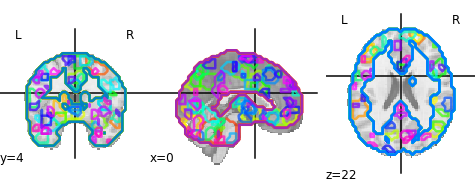
\includegraphics[width=0.8\linewidth]{atlas}
\captionof{figure}{ROIs highlighted on Craddock atlas}
\end{center}

\begin{enumerate}\compresslist
	\item Generated correlation matrices from pre-processed fMRIs
	\item Trained different LR and SVM models using Nested and Repeated 5-fold Cross Validation
	\item Used Grid Search to find optimal regularization strength parameter (C)
	\item Tested separately on female-only and male-only samples
	\item Generated connectivity matrices
	\item Repeated from $3.$ with connectivity matrices
\end{enumerate}


\vspace{1em}
We were able to reach an average accuracy of around 0.57.

\begin{center}
	\begin{tabular}{l l l}
		\toprule
		\textbf{Model} & \textbf{Train Acc.} & \textbf{Test Acc.}\\
		\midrule
		Log. Regression & 0.80 & 0.57 \\
		SVM & 0.91 & 0.57 \\
		\bottomrule
	\end{tabular}
	\captionof{table}{Final model performances obtained}
\end{center}

\end{multicols}
}

%----------------------------------------------------------------------------------------
%	REFERENCES
%----------------------------------------------------------------------------------------

\headerbox{References}{name=references,column=0,above=bottom}{

\renewcommand{\section}[2]{\vskip 0.05em} % Get rid of the default "References" section title
\nocite{*} % Insert publications even if they are not cited in the poster
\small{ % Reduce the font size in this block
\bibliographystyle{unsrt}
\bibliography{sample} % Use sample.bib as the bibliography file
}}

%----------------------------------------------------------------------------------------
%	FUTURE WORK
%----------------------------------------------------------------------------------------

\headerbox{Future Work}{name=futureresearch,column=1,span=2,aligned=references,above=bottom}{ % This block is as tall as the references block

\begin{multicols}{2}

As ASD diagnosis via Machine Learning remains an open problem, much is still to be done from a research point of view. Several are the classifiers we could try, but improvements in the future will highly depend on the amount of data that will be able to be collected from the research centers.

\end{multicols}
}

%----------------------------------------------------------------------------------------
%	CONTACT INFORMATION
%----------------------------------------------------------------------------------------

\headerbox{Code}{name=contact,column=3,aligned=references,above=bottom}{ % This block is as tall as the references block
\begin{description}\compresslist
	\item[Repo] https://github.com/GiuliaLo/MALIS-autism-diagnosis
\end{description}

}

%----------------------------------------------------------------------------------------
%	CONCLUSIONS
%----------------------------------------------------------------------------------------

\headerbox{Conclusions}{name=conclusion,column=2,span=2,row=0,below=results,above=references}{

\begin{multicols}{2}

\hspace{5.0em}
\begin{center}
	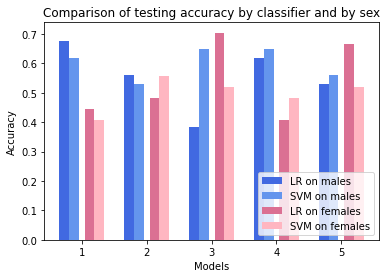
\includegraphics[width=1.0\linewidth]{histogram1}
	\captionof{figure}{Final comparisons results}
\end{center}


%------------------------------------------------

\begin{itemize}\compresslist
\item We tried both with the correlation matrices and the connectivity matrices as features, but we couldn't see significant differences between the two.
\item Having a small quantity of data for our testing set influenced our performance: we could see that from the testing results over the respective sexes varying significantly.
\end{itemize}

\end{multicols}
}

%----------------------------------------------------------------------------------------
%	METHODS
%----------------------------------------------------------------------------------------

\headerbox{Methods}{name=method,column=0,below=introduction,bottomaligned=conclusion}{ % This block's bottom aligns with the bottom of the conclusion block

The following Machine Learning methods were applied in our project:

\begin{itemize}\compresslist
\item Logistic Regression
\item Lasso Regularizer (L1)
\item Support Vector Machine
\item (k-fold) Cross Validation
\item Hyperparameter Grid Search
\end{itemize}\

Estimation of Logistic Regression parameters:

\begin{multline}
$$
\hat{w}_0, \hat{w} = arg_w min -\sum_{i=1}^{N} y_i log\sigma(w_0 + w^T x_i) + \\
(1 - y_i)log(1-\sigma(w_0 + w^T x_i))
$$
\end{multline}\


L1 Regularizer Function:

\begin{equation}
R(w) = \sum_{i=1}^{D} |w_i|
\end{equation}


}

%----------------------------------------------------------------------------------------
%	INITIAL RESULTS
%----------------------------------------------------------------------------------------

\headerbox{Initial Results}{name=results2,column=1,below=objectives,bottomaligned=conclusion}{ % This block's bottom aligns with the bottom of the conclusion block

We carried out our work over multi-site data obtained through the \textbf{ABIDE-II project}, focusing on resting-state fMRI scans of a 403 subjects filtered subset (balanced M/F and ASD/Control ratio, IQ and Age outliers removed).\\

Initially, we applied a pre-processing step to the images by using the \textbf{Configurable Pipeline for the Analysis of Connectomes (CPAC)}, obtaining for each subject higher quality brain scans, and analytical data such as the connectivity matrixes between Regions of Interest (ROIs) associated with several atlases.\\

An initial 5-fold cross-validated training over the Craddock matrixes resulted in overfitted models:


}

%----------------------------------------------------------------------------------------

\end{poster}

\end{document}